This chapter presents the user interface design of Students\&Companies, focusing on its structure and functionality to cater to students, companies and universities.
The objective of the design is to create a seamless, intuitive and efficient user experience.
To achieve this, it adheres to core principles that enhance simplicity, accessibility and consistency throughout the platform.

Ensuring consistency across the system, the design employs uniform fonts, colors and layouts, allowing users to navigate with ease and confidence.
Accessibility is a key tenet, with the interface accommodating users with disabilities and ensuring responsiveness across devices by adhering to Web Content Accessibility Guidelines (WCAG).
Finally, simplicity drives the design process, prioritizing logical workflows that minimize user effort and facilitate task completion.

\section{Flow Diagram}
The flow diagram below serves as a map of the platform's pages, illustrating their interconnections.
It provides a unified view to highlight overlaps and parallelisms across the functionalities for students, companies and universities.
This approach underscores the distinct aspects of the navigation while emphasizing its coherence.

\begin{figure}[h]
    \centering
    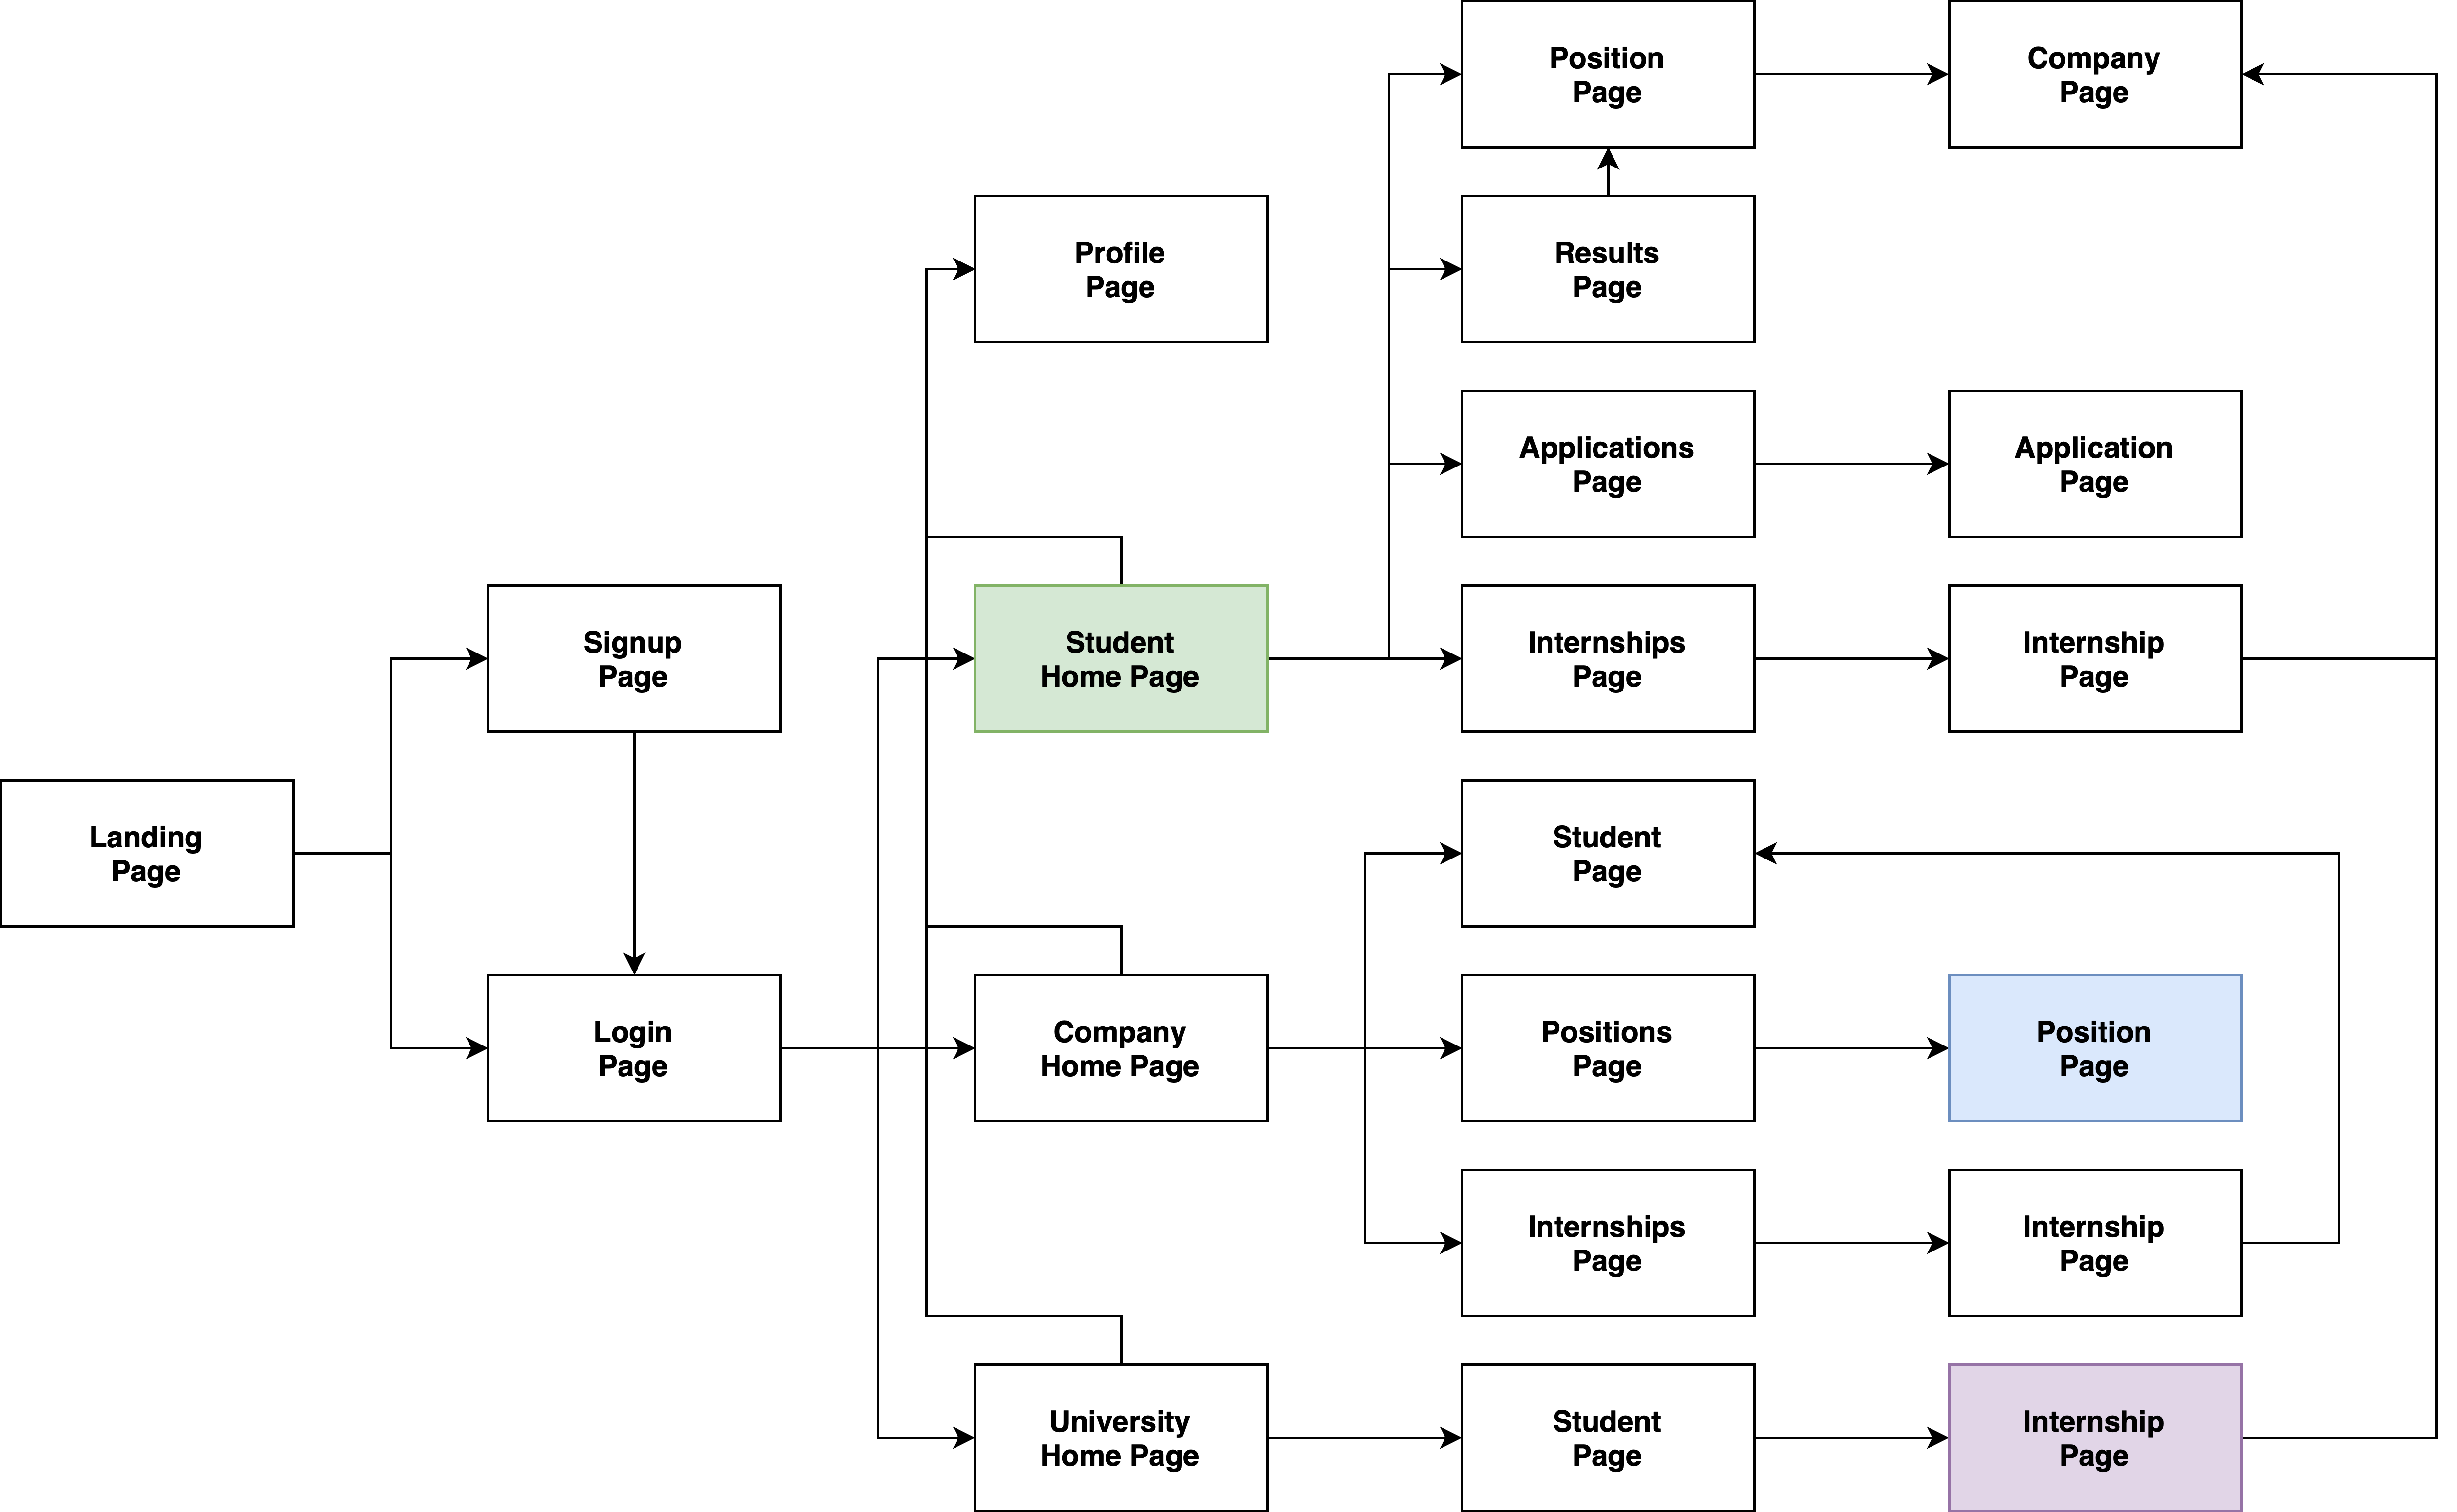
\includegraphics[width=16cm]{images/flow-diagram.png}
    \caption{Flow diagram}
\end{figure}

All primary pages of the platform are represented in this diagram, providing an overview of the core user workflows.
To maintain clarity, some finer details, such as the profile and questionnaire editors, interview page, feedback and comment forms, have been omitted but are mentioned in the requirements analysis and specification document \cite{carraracurrodossi2024}.
The pages highlighted in the diagram will be discussed in detail in the next section as they have been chosen as representative examples that showcase both the functionalities and the needs of each user category.

\section{Selected Pages}
The following section focuses on a selection of key pages within the platform.

\newpage
\subsection{Student Homepage}
The student homepage serves as the central hub for university students, designed to help them discover and apply for internship positions.
It features a header that includes links to the pages outlined in the flow diagram: the home, applications, internships and profile pages.
Note that this header is consistent across all of these pages, ensuring seamless navigation.
Similarly, the footer contains standard links such as privacy policy, terms of service and contact information, maintaining uniformity throughout the platform.

The main body of the homepage is focused on enabling students to search and explore positions.
It includes a search bar with filters for location, job type and field, allowing users to refine their results.
Below it, a list of recommendations is displayed.
Each position includes essential details such as location, job type and field, with options to expand for more information.
Students can view an expanded description of the position, along with clear buttons to either accept or reject the recommendation.

\begin{figure}
    \centering
    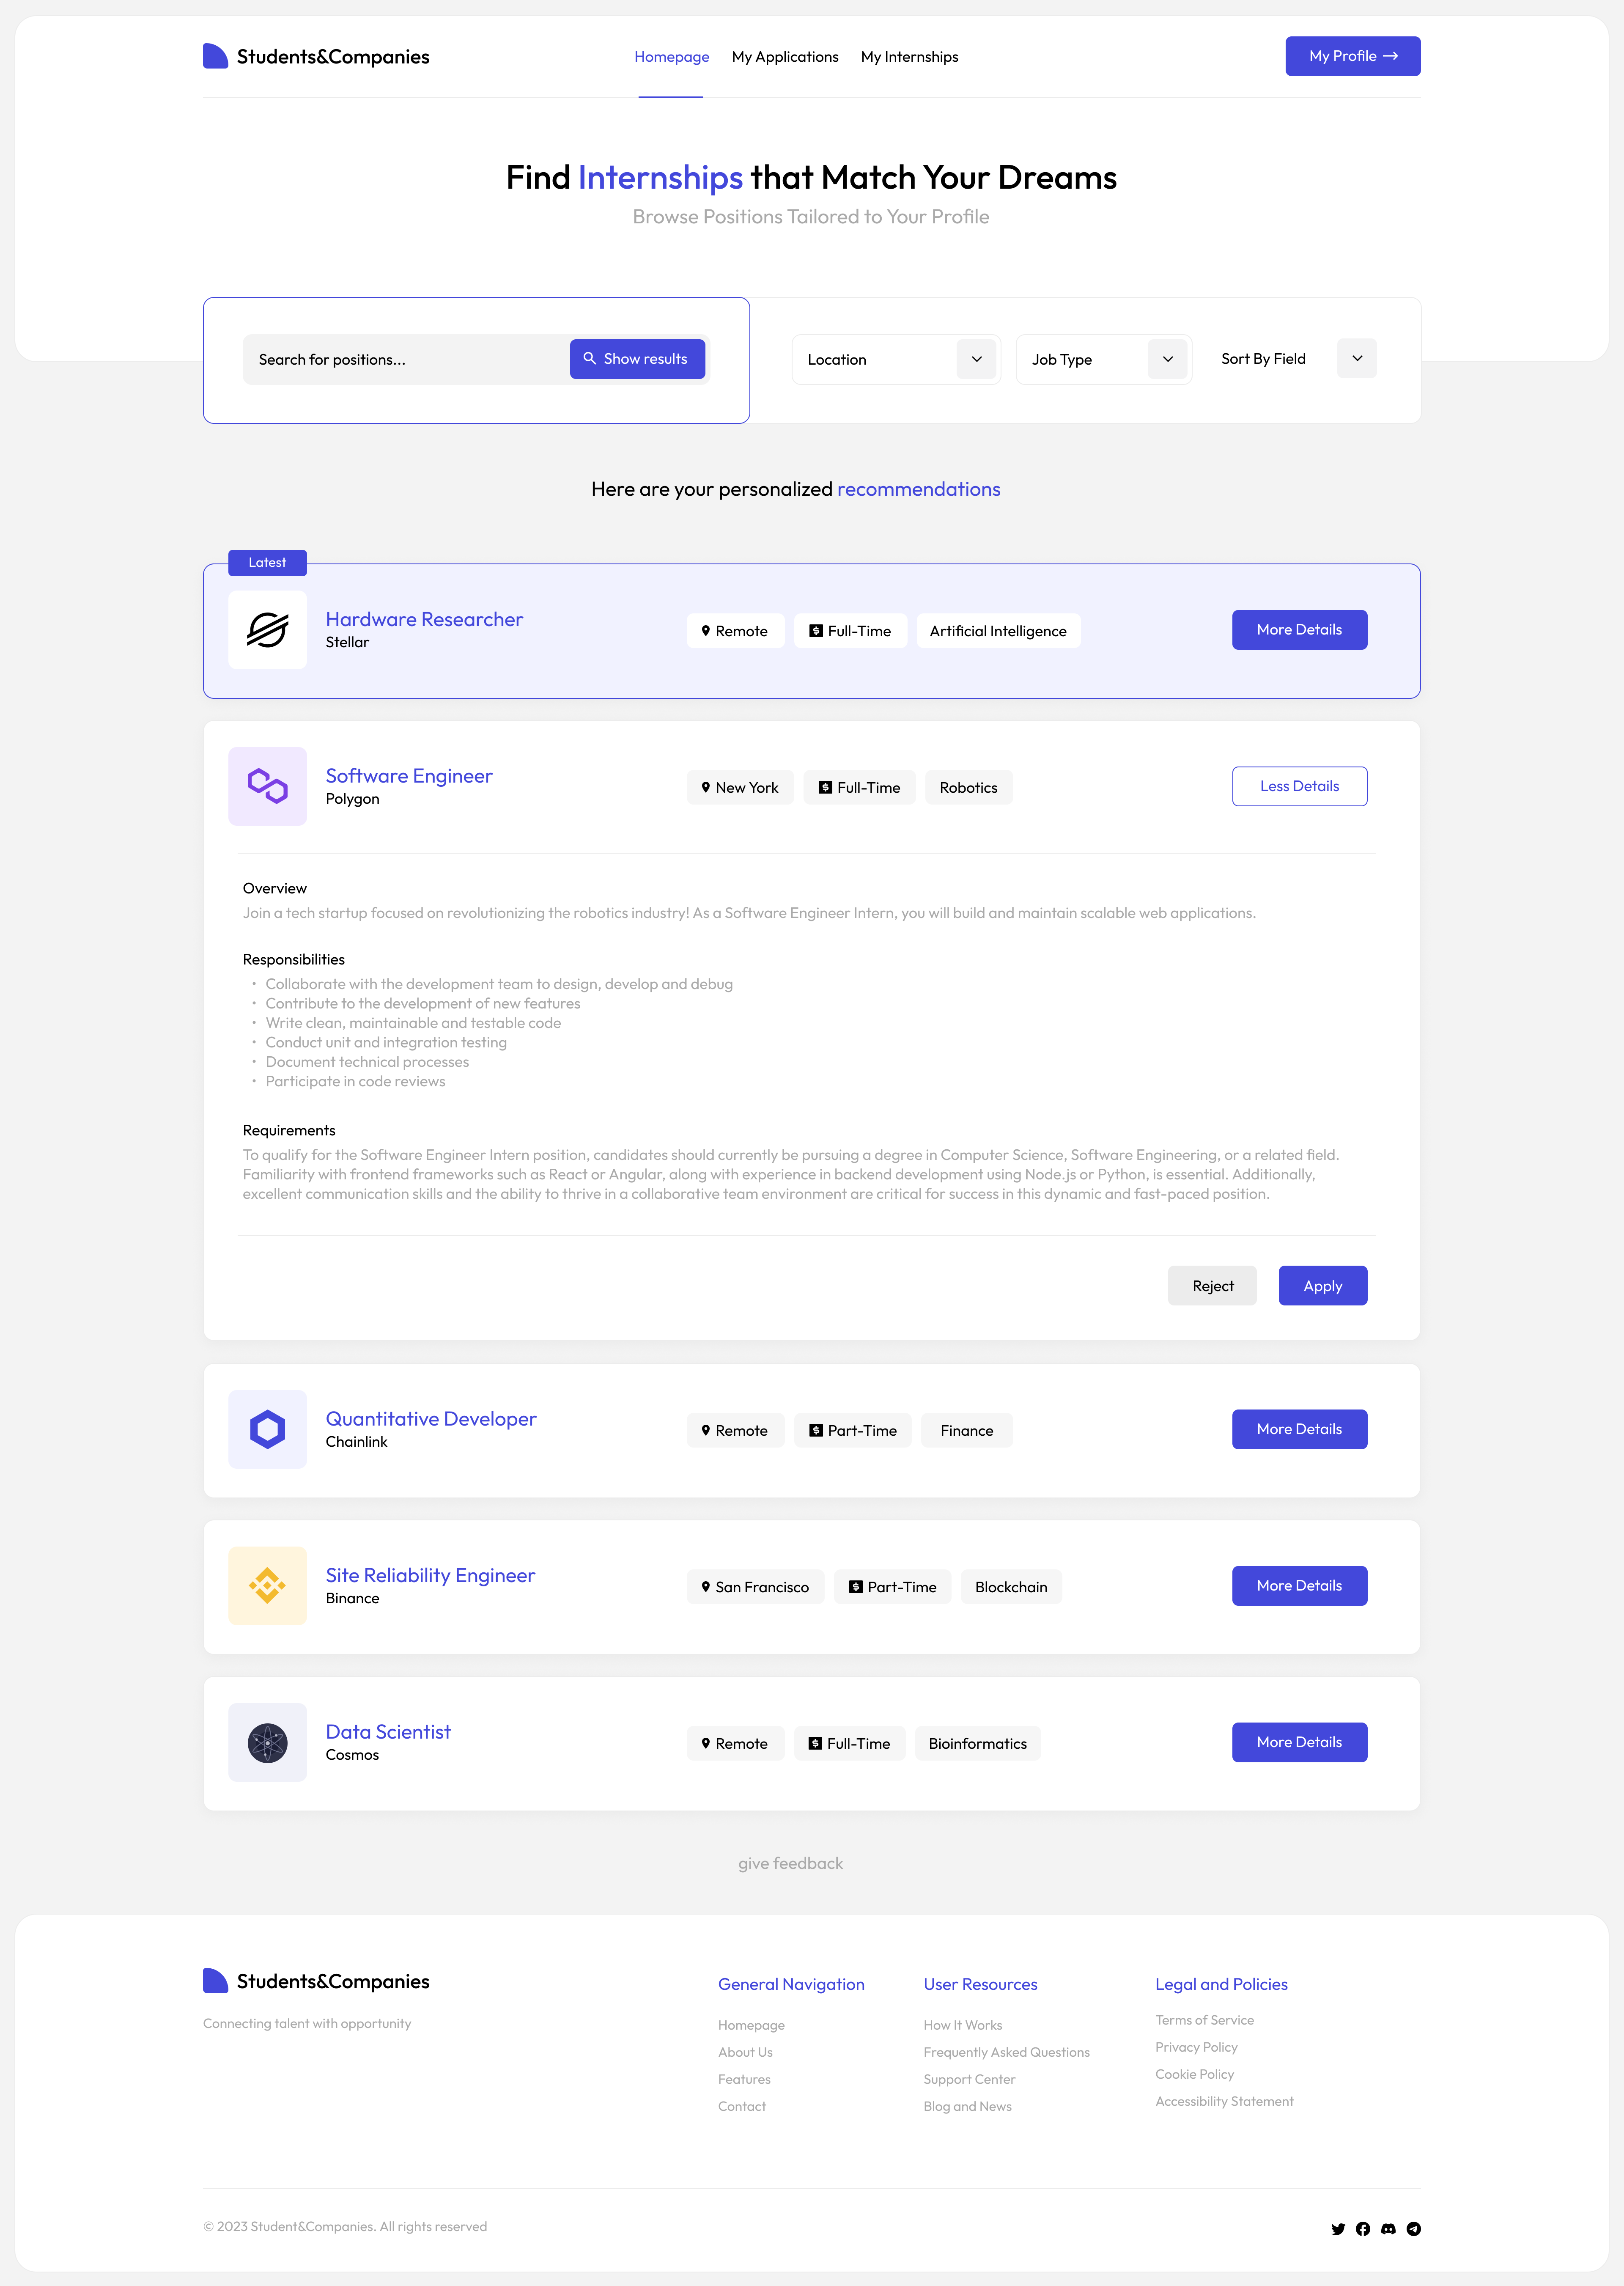
\includegraphics[width=15cm]{images/selected-pages/student-homepage.png}
    \caption{Student homepage}
\end{figure}

\subsection{Company Position Page}
The company position page maintains consistency with the platform's design through a familiar header and footer.
The body contains buttons for adding a questionnaire and scheduling an interview, with the date and time of the upcoming interview prominently displayed.
Below, it lists the questionnaires filled out by the student, which can be expanded to review answers.
Based on his performance, the company can either select or reject the candidate using the respective buttons, streamlining the selection process.

\begin{figure}
    \centering
    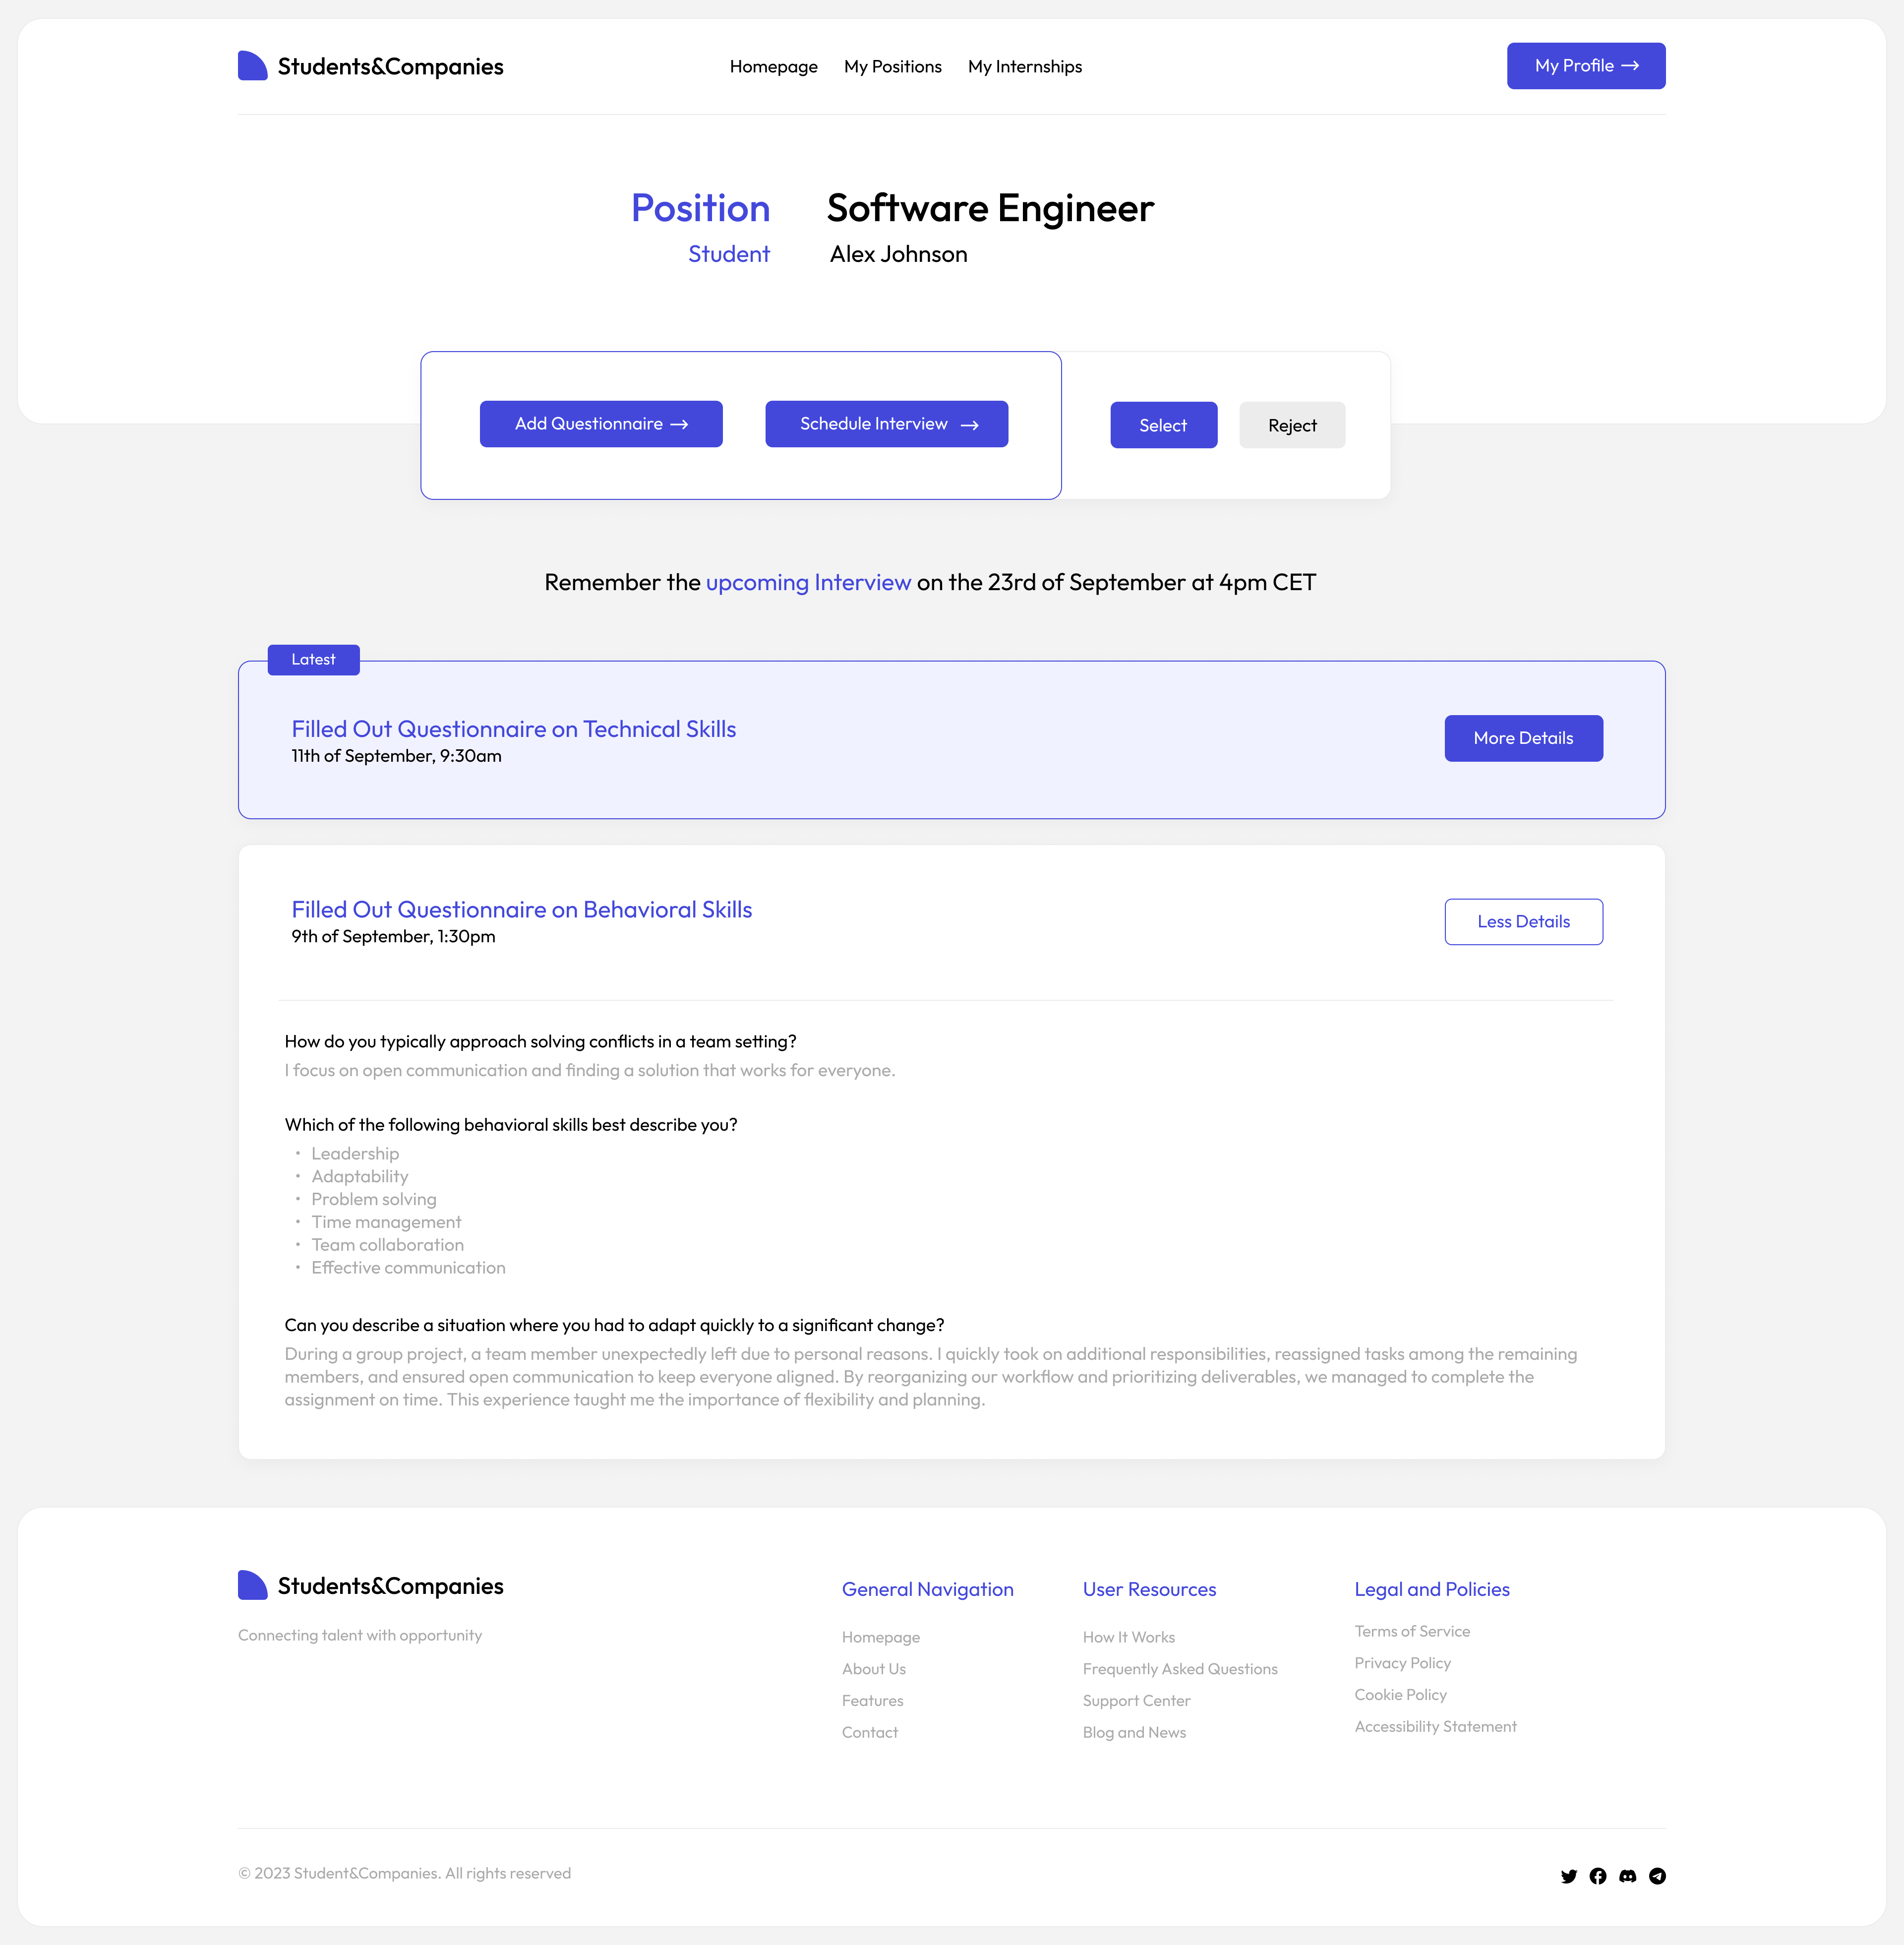
\includegraphics[width=16cm]{images/selected-pages/company-position-page.png}
    \caption{Company position page}
\end{figure}

\subsection{University Internship Page}
The university internship page ensures consistency with the platform through a standardized header and footer design.
The body allows universities to view comments on the internship or write them to report progress or address concerns.
These are displayed in an organized list, where each entry can be expanded to review the full content.
This interface facilitates communication between students, companies and universities, ensuring internships remain productive and beneficial for all parties involved.

\begin{figure}[h]
    \centering
    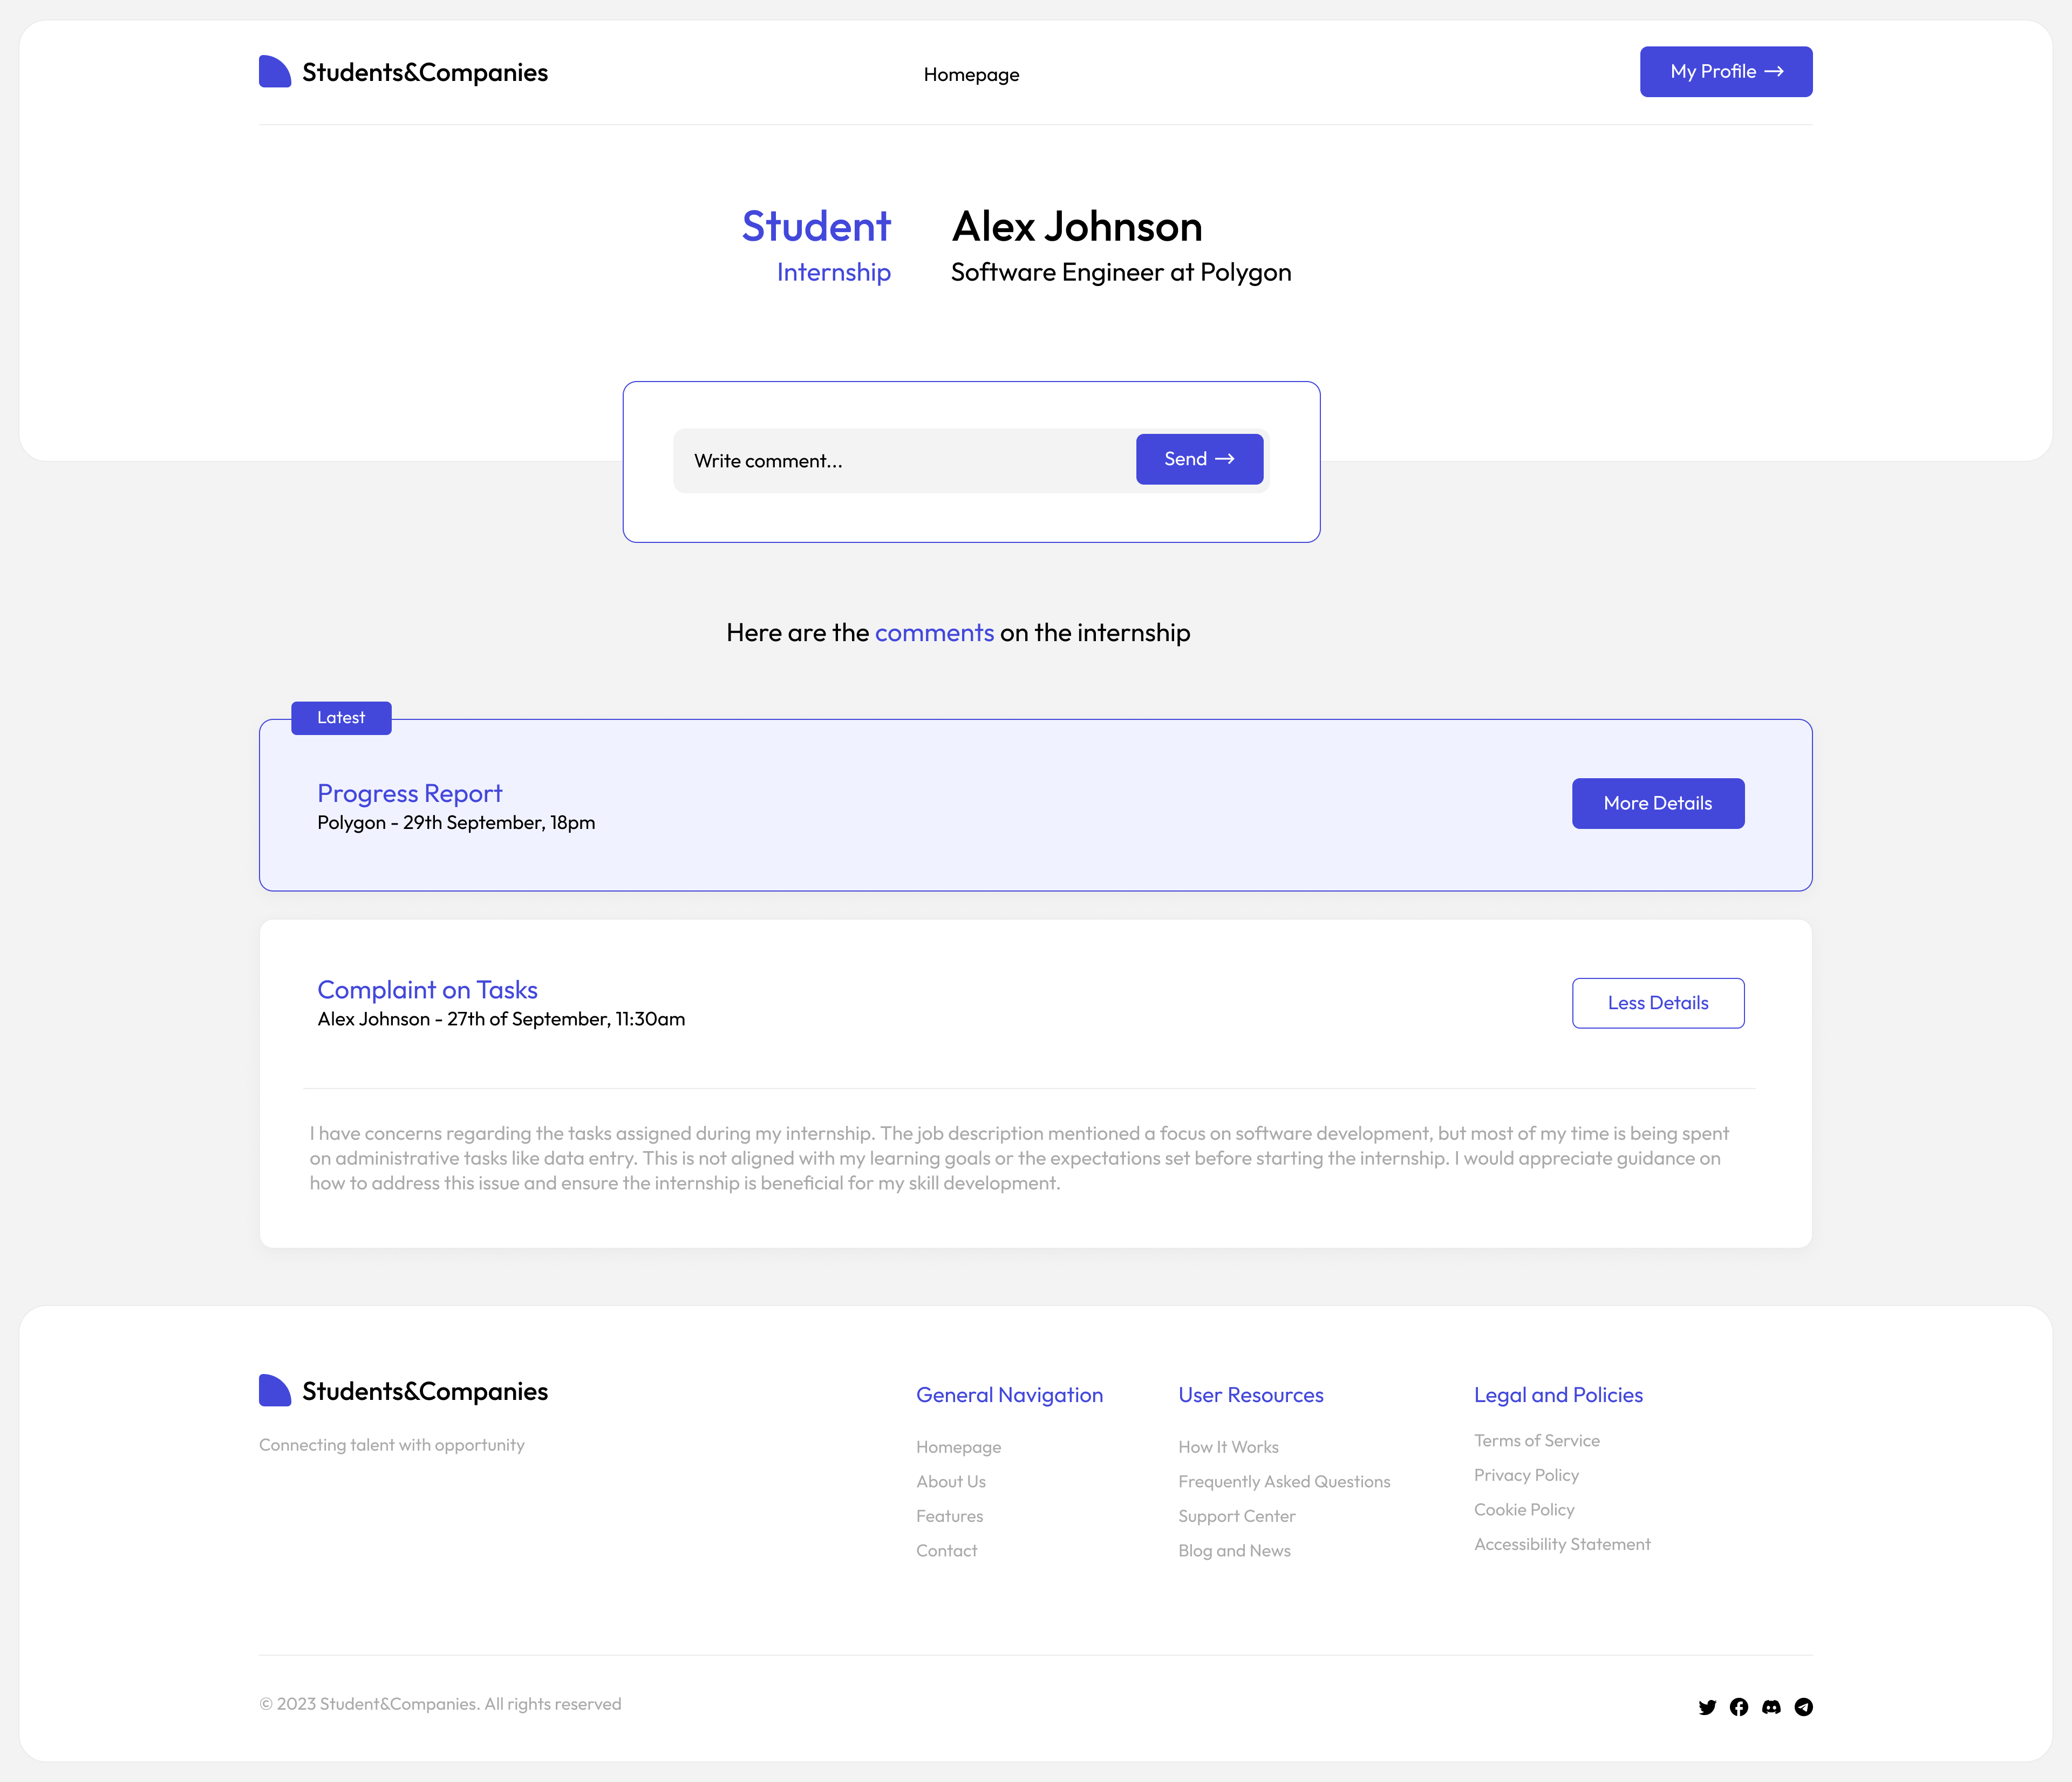
\includegraphics[width=16cm]{images/selected-pages/university-internship-page.png}
    \caption{University internship page}
\end{figure}
